\chapter{SonarQube}

\section{SonarQube}
\begin{enumerate}
    \item Start and install (first time) the \textit{SonarQube} instance with a docker image use the following command in you console: \begin{lstlisting}
        docker run -d --name sonarqube -e
        SONAR_ES_BOOTSTRAP_CHECKS_DISABLE=true -p 9000:9000
        sonarqube:latest
    \end{lstlisting}
    \item If the instance is running, you can login to \href{http://localhost:9000}{http://localhost:9000} and use the administrator credentials after the first login you need to change this credentials.
    \begin{lstlisting}
        login: admin
        password: admin
    \end{lstlisting}
    \item Create a new project with the name \textit{KubeWatch}
    \item Go to the \textit{KubeWatch} Project and choose locally analization.
    \item Generate a token (only first time) and safe this token somewhere you'll find it again (need it in the \textit{SonarScanner} section again).
    \item Choose Coninue and then choose other and your OS.
\end{enumerate}

\section{SonarScanner}
\begin{enumerate}
    \item Download the SonarScanner zip for your system from the following source: https://docs.sonarqube.org/latest/analysis/scan/sonarscanner/
    \item Extract the SonarScanner zip
    \item Add the bin folder in the extracted folder to the path variable (the location from the SonnarScanner folder doesn't depend).
    \item Adapt in the sonarscanner/conf folder the sonar-project.properties file with the following lines: \begin{lstlisting}
        #----- Local
        sonar.host.url=http://localhost:9000
        sonar.login=<your-sonar-qube-token>
        sonar.projectKey=KubeWatch
    \end{lstlisting}
    \item 
    \item Start SonnarScanner (scan) with the command: \begin{lstlisting}
        sh /<dir-path-to-sonnar-scanner-folder>/bin/sonar-scanner
    \end{lstlisting}
    (no error should be there)
    \item After the scan run, ther will be at the end of the console log a link to the actual report of the scan.
    \item If everything fine you'll get an scan overview like this: \newline
    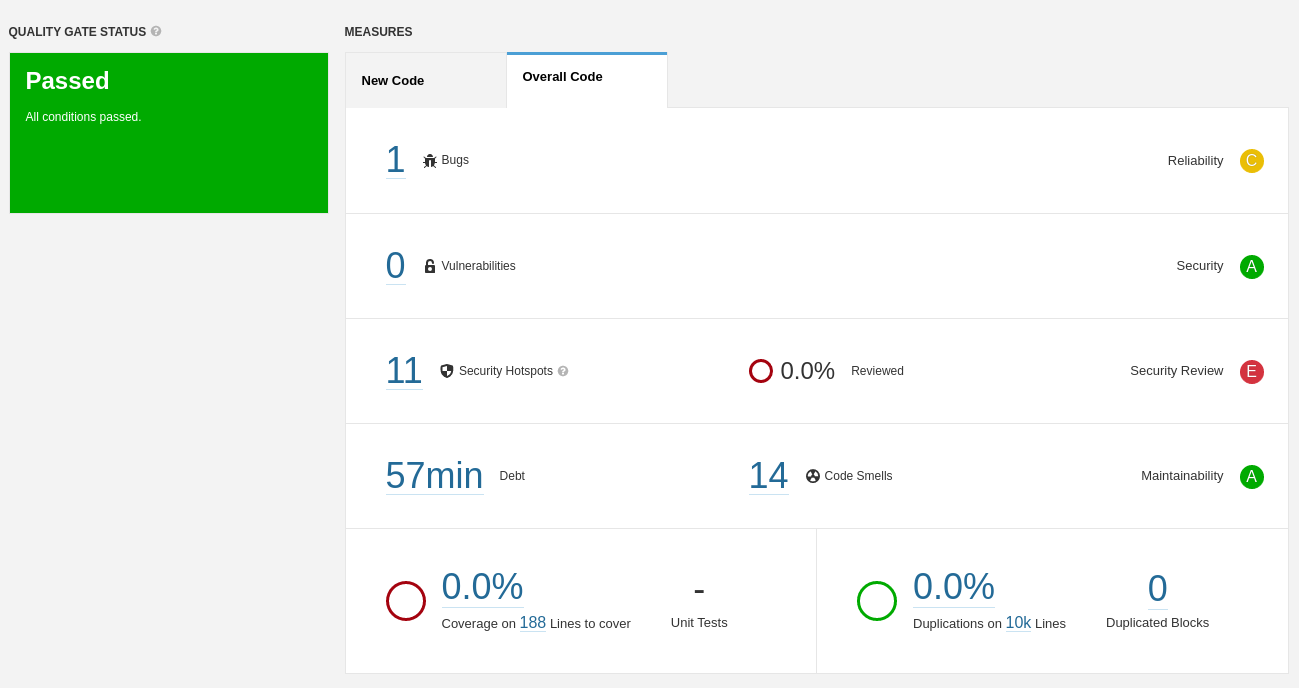
\includegraphics[height=8cm]{resources/scan.png}
\end{enumerate}

\section{Useful/Needed Docker Commands}
\subsection{Stop Docker Container}
After using SonarQube stop the local server with the following command
\begin{lstlisting}
    docker stop sonarqube
\end{lstlisting}

\subsection{Restart Docker Container}
To use the server again using the following command to restart the docker container:
\begin{lstlisting}
    docker restart sonarqube
\end{lstlisting}